%TC:macro \todomark [ignore]
%TC:macro \todoref [ignore]
%TC:macro \todocite [option:text,ignore]

% The above comments tell texcount that some macros should not have their arguments counted as text.
% \todomark, \todoref, and \todocite are all macros used during development - there will be no TODO messages
% in the final release.
% In particular, \todomark is sometimes used with long sentences e.g. \todomark{Should I use a different sentence here?} which I don't want to count.
% The \cref and \crefrange macros are used throughout the thesis, and are counted slightly incorrectly:
% While the actual output of \cref{hyp:cap_in_vec_load_store} = "Hyp. H-8" (2 or 3 words), TeXcount counts it as "hyp cap in vec load store" (6 words).
% This means the actual wordcount is an over-approximation.

%%%%%%%%%%%%%%%%%%%%%%%%%%%%%%%%%%%%%%%%%%%%%%%%%%%%%%%%%%%%%%%%%%%%%%%%%%%%%%%%
%% Introduction
%%
\chapter{Introduction\label{wc:start}\label{chap:intro}}
% PLAN: 1k words
% 2-3 pages

% \todomark{para on what capabilities are}
Since 2010, the Cambridge Computer Lab (in association with SRI) has been developing the CHERI\footnote{Capability Hardware Enhanced RISC Instructions} architecture extension, which improves the security of any given architecture by checking all memory accesses in hardware.
The core impact of CHERI, on a hardware level, is that memory can no longer be accessed directly through raw addresses, but must pass through a \emph{capability}\cite{TR-941}.
Capabilities are unforgeable tokens that grant fine-grained access to ranges of memory.
Instead of generating them from scratch, capabilities must be \emph{derived} from another capability with greater permissions.
For example, a capability giving read-write access to an array of structures can be used to create a sub-capability granting read-only access to a single element.
This vastly reduces the scope of memory-related security issues, such as buffer overflows\todocite{something something heartbleed?}, and creates interesting opportunities for software compartmentalization\todocite{CHERI: A Hybrid Capability-System Architecture for
Scalable Software Compartmentalization}.

Industry leaders have recognized the value CHERI provides.
Arm Inc have manufactured the Morello System-on-Chip, based on their Neoverse N1 CPU, which incorporates CHERI capabilities into the Armv8.2 ISA.
While this represents a great step forward, there are still elements on the SoC that haven't fully embraced CHERI (e.g. the GPU), and architecture extensions that haven't been investigated in the context of CHERI.
One such example is Arm's Scalable Vector Extension (introduced in Armv8.2 but not included in Neoverse N1), which is designed to remain in use well into the future\cite{stephensARMScalableVector2017}.
Supporting this and other scalable vector ISAs in CHERI is essential to CHERI's long-term relevance.

% \todomark{para on what vectors are}
In the context of modern computer architecture, vector processing is the practice of dividing a large hardware register into a \emph{vector} of multiple \emph{elements} and executing the same operation on each element in a single instruction\footnote{This is a SIMD (Single Instruction Multiple Data) paradigm.}.
This data-level parallelism can drastically increase throughput, particularly for arithmetic-heavy programs.
\todomark{explain Scalable vectors}
However, before computing arithmetic, the vectors must be populated with data.
% This is typically done using specialized vector memory accesses, which access a whole vector's worth of memory in a single instruction.

% This was the initial motivation for investigating the interactions between CHERI and vector processing.

% \todomark{above paras should explain why the interactions between the two are interesting}

\section{Motivation}
% \todomark{vectorized memory accesses required for vectorized arithmetic}
Modern vector implementations all provide vector load/store instructions to access a whole vector's worth of memory.
These range from simple contiguous accesses (where all elements are next to each other), to complex indexed accesses (where each element loads from a different location based on another vector).
They can also have per-element semantics, e.g. ``elements must be loaded in order, so if one element fails the preceding elements are still valid''\todocite{RISC-V V fault-only-first}.
% \todomark{Necessary for CHERI support in order for CHERI performance to be competitive}
If CHERI CPUs want to benefit from vector processing's increased performance and throughput, they must support those instructions at some level.
But adding CHERI's bounds-checking to the mix may affect these semantics, and could impact performance (e.g. checking each element's access in turn may be slow).

% \todomark{if this were the only priority, vectorized memory access doesn't need to be that fast relative to arithmetic?}
Vector memory access performance is more critical than one may initially assume, because vectors are used for more than just computation.
% \todomark{memcpy is a very common operation, vectorized on many platforms (cite)}
A prime example is \code{memcpy}: for \code{x86\_64}, \code{glibc} includes multiple versions of the function\footnote{It appears memcpy is implemented as a copy of memmove.} taking advantage of vector platforms, then selects one to use at runtime\footnote{\gitfile{sysdeps/x86_64/multiarch/ifunc-memmove.h}{bminor/glibc}{https://github.com/bminor/glibc/blob/7b1cfba79ee54221ffa7d7879433b7ee1728cd76/sysdeps/x86_64/multiarch/ifunc-memmove.h}}.
% \todomark{thus memory accesses themselves should be optimized}
These implementations are written in assembly and heavily optimized.
If the memory accesses are hitting the cache, a few extra cycles of bounds-checking for each access could actually make a noticeable difference.

% \todomark{also raises the question of storing capabilities within vectors, which could be useful for revocation strategies as proposed in XYZ}
\code{memcpy} also raises the important question of how the vector model interacts with capabilities.
In non-CHERI processors, \code{memcpy} will copy pointers around in memory without fuss.
For a CHERI-enabled vector processor to support this, it would need to be able to load/store capabilities from vectors without violating any security guarantees.
This may require more guarantees than otherwise necessary - for example, each vector register likely needs to be as large or larger than a single capability.

% \todomark{rvv introduces vectors for RVV}
% \todomark{rvv is scalable vector}
% \todomark{why rvv and not just arm}
% \todomark{CHERI has a RISC-V ISA + various implementations, wants to support vectors}
% \todomark{scalable vector support useful for future Arm support}
% \todomark{Current Morello doesn't support Arm SVE/NEON (cite?) despite the base Neoverse N1 supporting it (cite??)}
To explore this topic, we chose to focus on the RISC-V Vector extension (shortened to RVV throughout this dissertation, and specified in \cite{RISCVVectorExtension2021}).
As of November 2021 this has been ratified by RISC-V International\todocite{https://wiki.riscv.org/display/HOME/Recently+Ratified+Extensions}, and will be RISC-V's standard vector instruction set moving forward.
Choosing it has two key benefits.
Firstly, the CHERI project maintains three open-source cores (Piccolo, Flute, and Tooba\todocite{cheri risc-v page?}) implementing CHERI-RISC-V, none of which support vector processing.
Studying RVV will allow reference \enquote{CHERI-RVV} implementations to be built for these cores.
Secondly, RVV is a \emph{scalable} vector model.
This has more potential roadblocks than a fixed-length vector model, and investigating them here will make life easier if Arm wish to integrate their Scalable Vector Extension with CHERI later down the road.

% \section{Aims}
% The aim of this project is to investigate the impact of, and the roadblocks for, integrating a scalable vector architecture with CHERI's memory protection system.
% In particular, we focus on integrating RVV with the CHERI-RISC-V ISA, with the aim of enabling a future CHERI-RVV implementation and informing the approach for a future CHERI Arm SVE implementation.

% % Investigate the reprecussions of adding scalable vector support to CHERI systems.
% % \todomark{Identify where potential roadblocks could be, and where they couldn't be.}
% % What are potential performance/compatibility roadblocks?
% This project does not try to implement CHERI-RVV in a hardware description language.
% Instead, it uses an emulator written in Rust to experiment with potential integration methods.
% A higher-level approach allows us to evaluate what's plausible for hardware without getting stuck in the weeds of implementing it in full.

% % \todomark{Investigate from both hardware and software perspectives}
% Software and the user story for writing CHERI-RVV programs is also considered. 
% Where possible, vector code is generated from C source code using the CHERI-Clang compiler, rather than hand-writing assembly.
% This reveals many problems CHERI-Clang has with vector intrinsics, which we later propose solutions to.

% % \todomark{Investigate from both (adding CHERI to vector) and (adding vectors to CHERI) perspectives}
% As scalar CHERI processors and vector non-CHERI processors both already exist, we consider integration from both sides: how does vector processing change when adding CHERI, and how does CHERI change when adding vectors?
% Examples of these perspectives include the following:
% \begin{itemize}
%     \item When adding CHERI to vectors, do vectors need to be able to hold capabilities? If so, what changes are necessary?
%     \item When adding vectors to scalar CHERI, what are the benefits/drawbacks of using a separate hardware vector unit vs. an integrated scalar+vector pipeline?
% \end{itemize}

% % How does CHERI impact vector implementations (i.e. storing capabilities inside vectors for generic memcpy)
% % How do vectors impact CHERI implementations (particularly scalable vectors?)

\section{Hypotheses and Aims}
The goal of this project is to investigate the impact of, and the roadblocks for, integrating a scalable vector architecture with CHERI's memory protection system.
In particular, we focus on integrating RVV with the CHERI-RISC-V ISA, with the aim of enabling a future CHERI-RVV implementation and informing the approach for a future CHERI Arm SVE implementation.

The investigation was carried out by designing and testing a CHERI-RVV emulator written in Rust, but that is only a single implementation.
To show that RVV can be integrated with CHERI-RISC-V for a wide range of processors, we use information gathered from the emulator to prove \todomark{five} hypotheses (\cref{tab:hypotheses}).
\cref{hyp:hw_cap_as_vec_mem_ref,hyp:hw_cap_bounds_checks_amortized} take the point of view of the hardware, considering basic feasibility and potential performance issues.
\cref{hyp:sw_vec_legacy,hyp:sw_pure_compat,hyp:sw_stack_vectors,hyp:sw_multiproc} examine the current CHERI-RVV software stack, checking if adding CHERI to vector programs causes compatibility problems.
\cref{hyp:cap_in_vec_storage,hyp:cap_in_vec_load_store,hyp:cap_in_vec_manip} considers capabilities-in-vectors: the conditions under which vector registers can hold capabilities, and the conditions under which vectorized memory accesses and other instructions can manipulate them.

Along with testing these hypotheses, this document serves as a practical explanation of the following:
\begin{itemize}
    \item The changes to RISC-V required by CHERI-RISC-V
    \item The RISC-V-V vector model, and all memory-related instructions
    \item How to compile CHERI-RVV code for a baremetal platform (with no operating system)
    \item How to execute CHERI-RVV code compiled for a baremetal platform
    \item The limitations of the current CHERI-RVV software stack
\end{itemize}
\todomark{fill out this para more, have an actual end sentence}

\newcommand{\definehyp}[2]{{\sethyptext{#1}{#2}}\newhyp{}\label{#1} & #2}
\begin{table}[b]
    \centering
    \begin{tabular}{lp{0.9\linewidth}}
    \toprule
    \multicolumn{2}{l}{\emph{Hardware Hypotheses --- \cref{chap:hardware}}} \\
    \midrule
        \definehyp{hyp:hw_cap_as_vec_mem_ref}%
            {It is possible to use CHERI capabilities as memory references in all vector instructions.} \\
        \definehyp{hyp:hw_cap_bounds_checks_amortized}%
            {The cost of capability bounds checks can be amortised over multiple per-vector-element accesses.} \\
    \midrule
    \multicolumn{2}{l}{\emph{Software Hypotheses --- \cref{chap:software}}} \\
    \midrule
        \definehyp{hyp:sw_vec_legacy}%
            {Vector code can be compiled in legacy forms (with integer addressing) and still function correctly on CHERI with no source code changes.} \\
        \definehyp{hyp:sw_pure_compat}%
            {Vector code can be compiled into a pure-capability form from a legacy form with no source code changes.} \\
        \definehyp{hyp:sw_stack_vectors}%
            {Vector code that saves/restores variable-length vectors to/from the stack can be compiled on CHERI-RVV with no source code changes.} \\
        \definehyp{hyp:sw_multiproc}%
            {CHERI-vector code can run correctly in multiprocessing systems, where execution may be paused and resumed on interrupts or context switches.} \\
    \midrule
    \multicolumn{2}{l}{\emph{Capabilities-in-Vectors --- \cref{chap:capinvec}}} \\
    \midrule
        \definehyp{hyp:cap_in_vec_storage}%
            {It is possible for vector registers to hold capabilities to enable copying without violating CHERI's security principles.} \\
        \definehyp{hyp:cap_in_vec_load_store}%
            {It is possible for vector memory accesses to load and store capabilities from vector registers without violating CHERI's security principles.} \\
        \definehyp{hyp:cap_in_vec_manip}%
            {It is possible for vector instructions to manipulate capabilities in vector registers without violating CHERI's security principles.} \\
    \bottomrule
    \end{tabular}
    \caption{Project Hypotheses}%
    \label{tab:hypotheses}
\end{table}


%%%%%%%%%%%%%%%%%%%%%%%%%%%%%%%%%%%%%%%%%%%%%%%%%%%%%%%%%%%%%%%%%%%%%%%%%%%%%%%%
%% Background
%%
\chapter{Background}
% PLAN: 4k words

This chapter describes CHERI (\cref{chap:bg:sec:cheri}) and RVV (\cref{chap:bg:sec:rvv}) to the detail required to understand the rest of the dissertation.
Both are described because this dissertation caters to multiple audiences: those who already understand CHERI, but are less familiar with vectors; and those already familiar with vector hardware but not with CHERI.
The final section describes two other vector models in a little more detail.
They are both proprietary, so we cannot learn from their hardware, but they are useful for contextualizing the software side of things.


\section{CHERI}\label{chap:bg:sec:cheri}
% Concept of a capability
In CHERI, addresses/pointers are replaced with capabilities: unforgeable tokens that provide \emph{specific kinds of access} to an \emph{address} within a \emph{range of memory}.
The above statement is enough to understand what capabilities contain\footnote{This is a slight simplification. For the purposes of vector memory accesses the \emph{otype} of a capability can be ignored, as any type other than \code{UNSEALED} cannot be dereferenced anyway.}:
\begin{itemize}
    \item Permission bits, to restrict access
    \item The \emph{cursor}, i.e. the address it currently points to
    \item The \emph{bounds}, i.e. the range of addresses this capability could point to
\end{itemize}
A great deal of work has gone into compressing capabilities down into a reasonable size (see \cite{woodruffCHERIConcentratePractical2019}, \todoref{diagram from TR-941?}), and using the magic of floating-point all of this data has been reduced to just 2x the architectural register size.
For example, on 64-bit RISC-V a standard capability is 128-bits long.
The rest of this dissertation assumes capabilities are 128-bits long for simplicity.

In order to keep track of what is and isn't a valid capability, registers and memory are both tagged.
Each 128-bit register and each aligned 128-bit region of memory has an associated tag bit, which denotes if its data encodes a valid capability\footnote{This has the side-effect that capabilities must be 128-bit aligned in memory.}.
If any non-capability data is written to any part of the region, the tag bit is zeroed out.
\todomark{Can you have a capability with tag=1, but the cursor is outside the bounds?}
As above, significant work has gone into the implementation to reduce the DRAM overhead of this method (see \cite{joannouEfficientTaggedMemory2017} for an example).


\todomark{Explain the three security properties from davisCheriABIEnforcingValid2019?}


\todomark{rewrite above section - just copied over some stuff previously from Emulation Investigation and it doesn't flow}


\subsection{CHERI-RISC-V ISA}
The Cambridge Computer Lab's TR-951 report\todocite{TR-951} describes the latest version of the CHERI architecture (CHERI ISAv8) and proposes applications to MIPS, x86-64, and RISC-V.
CHERI-RISC-V is a mostly straightforward set of additions to basic RISC-V ISAs.
It adds thirty-two general-purpose capability registers, thirty-two Special Capability Registers (SCRs), and many new instructions.

The new general-purpose capability registers are each of size \code{CLEN = 2 * XLEN} plus a tag bit.
These registers store compressed capabilities.
While there is always a logical distinction between the pre-existing \emph{integer} registers \code{x0-x31} and the \emph{capability} registers \code{cx0-cx31}, the architecture may store them in a Split or Merged register file.
A Split register file stores the integer registers separately from capability registers, so programs can manipulate them independently.
A Merged register file stores thirty-two registers of length \code{CLEN}, using the full width for the capability registers, and aliases the integer registers to the bottom \code{XLEN} bits.
Under a merged register file, writing to an integer register makes the capability counterpart invalid, so programs have to be more careful with register usage.

\todomark{diagram for split/merged register file?}

\todomark{All new CHERI instructions specify if their operands are integers or capabilities, and pull from the correct set of logical registers.}
\todomark{Non-CHERI enabled instructions default to integer representations, and in some cases can be switched to use capabilities using the Integer/Capability encoding mode flag}

Many of the new SCRs are intended to support the privileged ISA extensions for e.g. hypervisors or operating systems.
The emulator doesn't use these, so their SCRs are not listed here, but there are two highly relevant SCRs for all modes: the Program Counter Capability and the Default Data Capability.
The PCC supplements \todomark{replaces?} the program counter by adding more metadata, ensuring instruction fetches have the same security as normal loads and stores.


\subsection{Integer/Capability mode}
\todomark{Capability mode flag overrides behaviour of RISC-V }

\subsection{Capability Relocations}
\todomark{talk about ELF cap-relocs table, how they work and why}

%---------------------------------
%---------------------------------
%---------------------------------
\section{A brief history of vector processing}
Many vector implementations (Intel SSE/AVX, Arm's Advanced SIMD and Neon) use fixed-length vectors - e.g. 128-bit vectors which a program interprets as four 32-bit elements.
As the industry's desire for parallelism grew, new implementations had to be designed with longer vectors of more elements.
For example, Intel SSE/SSE2 (both 128-bit) was succeeded by AVX (128 and 256-bit), then AVX2 (entirely 256-bit), then AVX-512 (512-bit).
Programs built for one extension, and hence designed for a specific vector size, could not automatically take advantage of longer vectors.

Scalable vectors address this by not specifying the vector length, and instead calculating it on the fly.
Instead of hardcoding \enquote{this loop iteration uses a single vector of four 32-bit elements}, the program has to ask \enquote{how many 32-bit elements will this iteration use?}.
This gives hardware designers more freedom, letting them select a suitable hardware vector length for their power/timing targets, while guaranteeing consistent execution of programs on arbitrarily-sized vectors.
RVV uses a scalable vector model.

\section{RVV}\label{chap:bg:sec:rvv}
% RISC-V has extensions
RISC-V is an open family of ISAs which defines ``base integer ISAs'' (e.g. all 64-bit RISC-V cores implement the RV64I Base Integer Instruction Set) and extensions (e.g. the ``M'' extension for integer multiplication).
A base instruction set combined with a set of extensions is known as a RISC-V ISA.
Because RISC-V is open, anyone can design, manufacture, and sell chips implementing any RISC-V ISA.
% RVV is the vector one
RVV is the officially ratified vector extension for RISC-V, and going forward all RISC-V chips with vector processing capabilities should implement it instead of designing their own custom vector extensions.
This section summarizes Sections 1-9 and 17 of the RVV Specification v1.0\cite{RISCVVectorExtension2021}.

%---------------------------------
%---------------------------------
%---------------------------------
\subsection{Vector model}\label{chap:bg:sec:rvv:vector_model}
\emph{Summarizes \cite[Sections 1-4]{RISCVVectorExtension2021}}
\todomark{Add prestart/active/inactive/body/tail definitions, would bump up to 1-5}


\figinput[width=0.7\textwidth,pos=h]{1_20Background/figures/fig_RVV_simple_widths}
\figinput[width=0.7\textwidth,pos=h]{1_20Background/figures/fig_RVV_added_state}


RVV defines thirty-two vector registers, each of an implementation-defined width VLEN.
These registers can be interpreted as \emph{vectors} of \emph{elements}.
The program can configure the size of elements, and the implementation defines a maximum width ELEN.
\cref{fig:RVV_simple_widths} shows a simple example of a 128-bit vector, where the maximum element length is 32-bits.


RVV also adds some state that defines how the vector registers are used (see \cref{fig:RVV_added_state}).
These are stored in RISC-V Control and Status Registers (CSRs), which the program can read.

%---------------------------------
\subsubsection{\code{vl} and \code{vstart}}\label{chap:bg:sec:rvv:vstart}
The first CSR is the Vector Length \code{vl}, which holds the number of elements that could be updated from a vector instruction.
The program updates this value through fault-only-first loads (\todoref{fof load}) and more commonly the \code{vsetvl} instruction family (\todoref{vsetvl}).

In the simple case, \code{vl} is equal to the total available elements (see \cref{fig:RVV_vl_full}).
It can also be fewer (see \cref{fig:RVV_vl_short}), in which case vector instructions will not write to elements in the \enquote{tail} (i.e. elements past \code{vl}).
This eliminates the need for a `cleanup loop' common in fixed-length vector programs.

\figinput[width=0.7\textwidth,pos=t]{1_20Background/figures/fig_RVV_vl}

In a similar vein, \code{vstart} specifies \enquote{the index of the first element to be executed by a vector instruction}.
This is usually only set by the hardware whenever it is interrupted mid-instruction (see \cref{fig:RVV_vstart_trap}) so that the instruction can be re-executed later without corrupting completed values.
Whenever a vector instruction completes, \code{vstart} is reset to zero.

The program \emph{can} set \code{vstart} manually, but it may not always work.
If an implementation couldn't arrive at the value itself, then it is allowed to reject it.
The specification gives an example where a vector implementation never takes interrupts during an arithmetic instruction, so it would never set \code{vstart} during an arithmetic instruction, so it could raise an exception if \code{vstart} was nonzero for an arithmetic instruction.

\figinput[width=0.7\textwidth,pos=t]{1_20Background/figures/fig_RVV_vstart_trap}

%---------------------------------
\subsubsection{\code{vtype}}
\code{vtype} contains two key fields that describe how vector instructions interpret the contents of vector registers.
The first is the Selected Element Width (\code{SEW}), which is self-explanatory.
It can be 8, 16, 32, or 64.
Most instructions\footnote{Except where the width is encoded in the instruction, like bytemask loads.} will split vector registers into elements of this width.

The second field is the Vector Register Group Multiplier (\code{LMUL}).
Vector instructions do not necessarily operate over a single register, but over a register \emph{group} as defined by this field.
For example, if \code{LMUL=8} then each instruction would operate over 8 register's worth of elements.
These groups must use aligned register indices, so if \code{LMUL=4} all vector register operands should be multiples of 4 e.g. \code{v0, v4, v8} etc.
In some implementations this may increase throughput, which by itself is beneficial for applications.

\figinput[width=0.7\textwidth,pos=t]{1_20Background/figures/fig_RVV_LMUL_widening}

However, the true utility of \code{LMUL} lies in widening/narrowing operations (see \cref{fig:RVV_LMUL_widening}).
For example, an 8-by-8-bit multiplication can produce 16-bit results.
Because the element size doubles, the number of vector registers required to hold the same number of elements also doubles.
Doubling \code{LMUL} after such an operation allows subsequent instructions to handle all the results at once.

\code{vtype} also encodes two flags: mask-agnostic and tail-agnostic.
If these are set, the implementation is \emph{allowed} to overwrite any masked-out or tail elements with all 1s.

Most vector instructions will interpret their operands using \code{vtype}, but this is not always the case.
Some instructions (such as memory accesses) use different Effective Element Widths (\code{EEW}) and Effective LMULs (\code{EMUL}) for their operands.
In the case of memory accesses, these are encoded in the instruction bits.
Another example is widening/narrowing operations, which by definition have to interpret the destination registers differently from the sources.

\pagebreak
\figinput[width=0.8\textwidth,pos=h]{1_20Background/figures/fig_RVV_mask_example}
%---------------------------------
\subsubsection{Masking}
Most vector instructions allow for per-element \emph{masking} (see \cref{fig:RVV_mask_example}).
When masking is enabled, register \code{v0} acts as the `mask register', where each bit corresponds to an element in the vector.
If the mask bit is 1, that element will be `masked out' and not written to (or depending on the mask-agnostic setting, overwritten with 1s).

\todomark{There will always be enough bits in a single register to mask all elements. maximum element count comes from smallest SEW (8 bits) and largest LMUL (8 registers). Max elements = VLEN * LMUL / SEW = VLEN * 8 / 8 = VLEN elements, there are VLEN bits in a single register.}

\figinput[width=\textwidth,pos=h]{1_20Background/figures/fig_RVV_examples_combined}
%---------------------------------
\subsubsection{Summary}
\cref{fig:RVV_examples_combined} shows all of the above features used in a single configuration:
\begin{itemize}
    \item The instruction was previously interrupted and restarted, so \code{vstart=2}
    \item Elements are 16-bit
    \item \code{LMUL=4} to try and increase throughput
    \item Only 29 of the 32 available elements were requested, so \code{vl=29}
    \item Some elements are masked out (in this case seemingly at random)
\end{itemize}

\pagebreak
%---------------------------------
%---------------------------------
%---------------------------------
\subsection{Strip mining and \code{vsetvl}}
\emph{Summarizes \cite[Section 6]{RISCVVectorExtension2021}}
\todomark{example usage of the above, introduces vsetvli}

\pagebreak
%---------------------------------
%---------------------------------
%---------------------------------
\subsection{Exception handling}
\emph{Summarizes \cite[Section 17]{RISCVVectorExtension2021}}

During the execution of a vector instruction, two events can prevent an instruction from fully completing: a synchronous exception in the instruction itself, or an asynchronous interrupt from another part of the system.
Implementations may choose to wait until an instruction fully completes before handling asynchronous interrupts, making it unnecessary to pause the instruction halfway through, but synchronous exceptions cannot be avoided in this way (particularly for those performing memory accesses).
The RVV specification defines two modes for `trapping' these events, which implementations may choose between depending on the context (e.g. the offending instruction), and notes two further modes which may be used in further extensions.
All modes start by saving the PC of the trapping instruction to a CSR \code{*epc}.

%---------------------------------
\subsubsection{Imprecise vector traps}
Imprecise traps are intended for events that are not recoverable, where \enquote{reporting an error and terminating execution is the appropriate response}.
They do not impose any extra requirements on the implementation.
For example, an implementation that executes instructions out-of-order does not need to guarantee that instructions older than \code{*epc} have completed, and is allowed to have completed instructions newer than \code{*epc}.

If the trap was triggered by a synchronous exception, the \code{vstart} CSR must be updated with the element that caused it.
\todomark{inconsistency in spec - Ch17 first para says "the vstart CSR contains the element index on which the trap was taken", but the imprecise trap section only specifies this for synchronous exceptions}

The specification also states \enquote{There is no support for imprecise traps in the current standard extensions}, \todomark{what does this mean?}

%---------------------------------
\subsubsection{Precise vector traps}
Precise vector traps are intended for instructions that can be resumed after handling the interrupting event.
This means the architectural state (i.e. register values) when starting the trap could be saved and reloaded before continuing execution.
Therefore it must look like instructions were completed in-order, even if the implementation is out-of-order:
\begin{itemize}
    \item Instructions older than \code{*epc} must have completed (committed all results to the architectural state)
    \item Instructions newer than \code{*epc} must \textbf{not} have altered architectural state.
\end{itemize}

On a precise trap, regardless of what caused it, the \code{vstart} CSR must be set to the element index on which the trap was taken.
The save-and-reload expectation then add two constraints on the trapping instruction's execution:
\begin{itemize}
    \item Operations affecting elements preceding \code{vstart} must have committed their results
    \item Operations affecting elements at or following \code{vstart} must either
    \begin{itemize}
        \item not have committed results or otherwise affected architectural state
        \item be \emph{idempotent} i.e. produce exactly the same result when repeated.
    \end{itemize}
\end{itemize}

The idempotency option gives implementations a lot of leeway.
Some instructions \todomark{examples} are specifically prohibited from overwriting their inputs to make them idempotent.
If an instruction is idempotent, an implementation is even allowed to repeat operations on elements \emph{preceding} \code{vstart}.
However for memory accesses the idempotency depends on the memory being accessed.
For example, writing to a memory-mapped I/O region may not be idempotent.

Another memory-specific issue is that of \emph{demand-paging}, where the OS needs to step in and move virtual memory pages into physical memory for an instruction to use.
This use-case is specifically called out by the specification for precise traps.
Usually, this is triggered by some element of a vector memory access raising a synchronous exception, invoking a precise trap, and \todomark{using \code{vstart} to show the OS which address it wants?}
Because \code{vstart} must be set to the element that demanded the page, and operations preceding \code{vstart} must have completed, any elements that could potentially trigger demand-paging \emph{must} wait for the preceding elements to complete.
This always applies, no matter what the instruction's specific ordering guarantees are.

%---------------------------------
\subsubsection{Other modes}
The RVV spec mentions two other potential trap modes.
First is \enquote{Selectable precise/imprecise traps}, where an implementation provides a bit that selects between precise or imprecise traps.
The intent is to allow precise traps to be selected for e.g. debugging purposes, and for imprecise traps to be selected for extra performance.

The second mode is \enquote{Swappable traps}, where a trap handler could use special instructions to \enquote{save and restore the vector unit microarchitectural state}.
The intent seems to be to support context switching with imprecise traps, which could also require the \emph{opaque} state (i.e. internal state not visible to the program) to be saved and restored.
Right now, it seems that context switching always requires a precise trap.

Neither of these modes are actually defined, but they are simply noted as possibilities for the future.

\pagebreak
%---------------------------------
%---------------------------------
%---------------------------------
\subsection{Memory access instructions}
\emph{Summarizes \cite[Sections 7-9]{RISCVVectorExtension2021}}

RVV defines five broad categories of memory access instructions, which this subsection describes.
For the most part, they handle their operands as described in \cref{chap:bg:sec:rvv:vector_model}.
\code{EEW} and \code{EMUL} are usually derived from the instruction encoding, rather than reading the \code{vtype} CSR.
In one case (\todoref{bytemask access}) the Effective Vector Length \code{EVL} is different from the \code{vl} CSR, so for simplicity all instructions are described in terms of \code{EVL}.

\subsubsection{Segment accesses}
Three of the five categories (unit/strided, fault-only-first, and indexed) support \emph{segmented} access.
This is used for unpacking contiguous structures of $n$ \emph{fields} and placing each field in a separate vector.
Rather than 

\pagebreak
\subsubsection{Unit and Strided accesses}


\begin{tabular}{ll}
\toprule
    \code{EEW} & From Instruction \\
    \code{EMUL} & From Instruction \\
    \midrule
    \code{NFIELDS} & From Instruction \\
    \code{EVL} & \code{vl} \\
    \bottomrule
\end{tabular}

\pagebreak
\subsubsection{Fault-only-first unit loads}

\begin{tabular}{ll}
\toprule
    \code{EEW} & From Instruction \\
    \code{EMUL} & From Instruction \\
    \midrule
    \code{NFIELDS} & From Instruction \\
    \code{EVL} & \code{vl} \\
    \bottomrule
\end{tabular}

\pagebreak
\subsubsection{Indexed accesses}
\begin{tabular}{ll}
\toprule
    Element \code{EEW} & \code{vtype.SEW} \\
    Element \code{EMUL} & \code{vtype.LMUL} \\
    \midrule
    Index Width & From Instruction \\
    Index \code{MUL} & From Instruction \\
    \midrule
    \code{NFIELDS} & From Instruction \\
    \code{EVL} & \code{vl} \\
    \bottomrule
\end{tabular}

\pagebreak
\subsubsection{Whole-register accesses}
\begin{tabular}{ll}
\toprule
    \code{EEW} & From Instruction \\
    \midrule
    \code{NFIELDS} & From Instruction \\
    \code{EVL} & \code{NFIELDS * VLEN / EEW} \\
    \bottomrule
\end{tabular}

\pagebreak
\subsubsection{Bytemask accesses}
\begin{tabular}{ll}
\toprule
    \code{EEW} & 8-bits \\
    \code{EMUL} & 1 \\
    \midrule
    \code{EVL} & \code{ceil(vl/8)} \\
    \bottomrule
\end{tabular}

\pagebreak
%---------------------------------
%---------------------------------
%---------------------------------
\subsection{Implementations}

\section{Other vector models}
\subsection{Arm SVE}
\subsection{Intel SSE/AVX}


%%%%%%%%%%%%%%%%%%%%%%%%%%%%%%%%%%%%%%%%%%%%%%%%%%%%%%%%%%%%%%%%%%%%%%%%%%%%%%%%
%% Main Chapter
%%
\documentclass[../thesis]{subfiles}
\begin{document}

\chapter{Hardware emulation investigation\label{chap:hardware}}
In order to experiment with integrating CHERI and RVV, we implemented a RISC-V emulator in the Rust programming language named \code{riscv-v-lite}.
The emulator can partially emulate four unprivileged\footnote{i.e. entirely bare-metal without privilege levels for OSs or hypervisors.} RISC-V ISAs (\cref{tab:emu_arches}), and was also used as the base for capabilities-in-vectors research (\cref{chap:capinvec}).
This chapter explores the development of the emulator, the implementation of CHERI support (including supplementary libraries), the addition of vector support, and the conclusions drawn about the integration of CHERI and RVV (referred to as CHERI-RVV throughout).

\begin{table}[h]
    \centering
    \begin{tabular}{cll}
    \toprule
    \multicolumn{2}{c}{Architecture} & Extensions \\
    \midrule
    32-bit & \code{rv32imv} & Multiply, CSR, Vector\parnote{Floating-point parts of the vector extension are not supported.\label{rvvnofloat}}  \\
    64-bit & \code{rv64imv} & Multiply, CSR, Vector\parnoteref{rvvnofloat}  \\
    64-bit & \code{rv64imvxcheri} & Multiply, CSR, Vector\parnoteref{rvvnofloat}, CHERI  \\
    64-bit & \code{rv64imvxcheri-int} & Multiply, CSR, Vector\parnoteref{rvvnofloat}, CHERI (Integer)  \\
    \bottomrule
    \end{tabular}
    \parnotes
    \caption{\code{riscv-v-lite} supported architectures}
    \label{tab:emu_arches}
\end{table}

\section{Developing the emulator}\label{chap:software:sec:emu}

The emulator for each architecture follows a similar pattern.
A \code{Processor} struct stores the register file and the available RAM.
A separate \code{ProcessorModules} struct holds all ISA modules the processor can execute (e.g. the base RV64 Integer ISA, the Multiply extension, and the Vector extension).

The gap between the \code{Processor} and the ISA modules is bridged by a module-specific ``connector'' struct, which holds references to data in the \code{Processor} that is required by the ISA module.
For example, the RV64 Integer ISA's connector contains the current PC, a virtual reference to a register file, and a virtual reference to memory.
This allows different \code{Processor} structs (e.g. a normal RV64 and a CHERI-enabled RV64) to reuse the same ISA modules despite using different register file implementations.

Each \code{Processor} implements a single stage pipeline.
Instructions are fetched, decoded with a common decoder function\footnote{The decoder, and therefore all emulated processors, doesn't support RISC-V Compressed instructions.}, and executed.
The processor asks each ISA module in turn if it wants to handle the instruction, and uses the first module to say yes.
If the ISA module returns a new PC value it is immediately applied, otherwise it is automatically incremented.
This structure easily represents basic RISC-V architectures, and can scale up to support many different new modules.

\subsection{Emulating CHERI}

Manipulating CHERI capabilities securely and correctly is a must for any CHERI-enabled emulator.
Capability encoding logic is not trivial by any means, so the \code{cheri-compressed-cap} C library was re-used rather than implementing it from scratch.
Rust has generally decent interoperability with C, but some of the particulars of this library caused issues.

\subsubsection{\code{rust-cheri-compressed-cap}}
\code{cheri-compressed-cap} provides two versions of the library by default, for 64-bit and 128-bit capabilities, which are generated from a common source through extensive use of the preprocessor.
Each variant defines a set of preprocessor macros (e.g. the widths of various fields) before including two common header files \code{cheri\_compressed\_cap\_macros.h} and \code{cheri\_compressed\_cap\_common.h}.
The latter then defines every relevant structure or function based on those preprocessor macros.
For example, a function \code{compute_base_top} is generated twice, once as  \code{cc64\_decompress\_mem} returning \code{cc64\_cap\_t} and another time as \code{cc128\_decompress\_mem} returning \code{cc128\_cap\_t}.
Elegantly capturing both sets was the main challenge for the Rust wrapper.

One of Rust's core language elements is the Trait - a set of functions and \enquote{associated types} that can be \emph{implemented} for any type.
This gives a simple way to define a consistent interface: define a trait \code{CompressedCapability} with all of the functions from \code{cheri\_compressed\_cap\_common.h}, and implement it for two empty structures \code{Cc64} and \code{Cc128}.
In the future, this would allow the Morello versions of capabilities to be added easily.
A struct \code{CcxCap<T>} is also defined which uses specific types for addresses and lengths pulled from a \code{CompressedCapability}.
For example, the 64-bit capability structure holds a 32-bit address, and the 128-bit capability a 64-bit address.

128-bit capabilities can cover a 64-bit address range, and thus can have a length of $2^{64}$.
Storing this length requires 65-bits, so all math in \code{cheri\_compressed\_cap\_common.h} uses 128-bit length values.
C doesn't have any standardized 128-bit types, but GCC and LLVM provide so-called ``extension types'' which are used instead.
Although the x86-64 ABI does specify how 128-bit values should be stored and passed as arguments\cite{specification-x86-psABI-v1.0}, these rules do not seem consistently applied\footnote{See \url{https://godbolt.org/z/qj43jssr6} for an example.}.
This causes great pain to anyone who needs to pass them across a language boundary.

Rust explicitly warns against passing 128-bit values across FFI, and the Clang User's Manual even states that passing \code{i128} by value is incompatible with the Microsoft x64 calling convention\footnote{\gitfile[release/13.x]{clang/docs/UsersManual.rst:3384}{llvm/llvm-project}{https://github.com/llvm/llvm-project/blob/release/13.x/clang/docs/UsersManual.rst\#x86}}.
This could be resolved through careful examination: for example, on LLVM 128-bit values are passed to functions in two 64-bit registers\footnote{\gitfile[release/13.x]{clang/lib/CodeGen/TargetInfo.cpp:2811}{llvm/llvm-project}{https://github.com/llvm/llvm-project/blob/75e33f71c2dae584b13a7d1186ae0a038ba98838/clang/lib/CodeGen/TargetInfo.cpp\#L2811}}, which could be replicated in Rust by passing two 64-bit values.
For convenience, we instead rely on the Rust and Clang compilers using compatible LLVM versions and having identical 128-bit semantics.

The CHERI-RISC-V documentation contains formal specifications of all the new CHERI instructions, expressed in the Sail architecture definition  language\footnote{\gitrepo{rems-project/sail}{https://github.com/rems-project/sail}}.
These definitions are used in the CHERI-RISC-V formal model\footnote{\gitrepo{CTSRD-CHERI/sail-cheri-riscv}{https://github.com/CTSRD-CHERI/sail-cheri-riscv}}, and require a few helper functions (see \cite[Chapter 8.2]{TR-951}).
To make it easier to port the formal definitions directly into the emulator the \code{rust-cheri-compressed-cap} library also defines those helper functions.

The above work is available online\footnote{\redact{\gitrepo{theturboturnip/cheri-compressed-cap}{https://github.com/theturboturnip/cheri-compressed-cap}}}, and includes documentation for all C functions (which is not documented in the main repository).
That documentation is also available online\footnote{\redact{\url{https://theturboturnip.github.io/files/doc/rust_cheri_compressed_cap/}}} and partially reproduced in \cref{appx:docs:rustcherilib}.

\subsubsection{Integrating into the emulator}
% i.e. using MemoryOf trait to make all memory addressable only by capabilities
Integrating capabilities into the emulator was relatively simple thanks to the modular emulator structure.
A capability-addressed memory type was created, which wraps a simple integer-addressed memory in logic which performs the relevant capability checks.
For integer encoding mode, a further integer-addressed memory type was created where integer addresses are bundled with the DDC before passing through to a capability-addressed memory (see \cref{fig:emulatormemory}).
% For integer encoding mode, a further integer-addressed memory type was created which wraps the capability addressed mode, where all integer addresses are bundled with the DDC before passing through to the capability-addressed memory.
Similarly, a merged capability register file type was created that exposed integer-mode and capability-mode accesses.
This layered approach meant code for basic RV64I operations did not need to be modified to handle CHERI at all --- simply passing the integer-mode memory and register file would perform all relevant checks.

% i.e. isn't the module system nice for overriding specific behaviour like Capability-mode RV64I :)
Integrating capability instructions was also simple.
Two new ISA modules were created: \code{XCheri64} for the new CHERI instructions, and \code{Rv64imCapabilityMode} to override the behaviour of legacy instructions in capability-encoding-mode (see \cref{fig:module_algorithm}).
The actual Processor structure was left mostly unchanged.
Integer addresses were changed to capabilities throughout,
memory and register file types were changed as described above, and the PCC/DDC were added.

\begin{figure}
    \centering
    \begin{minipage}[c]{.4\textwidth}
      \centering
      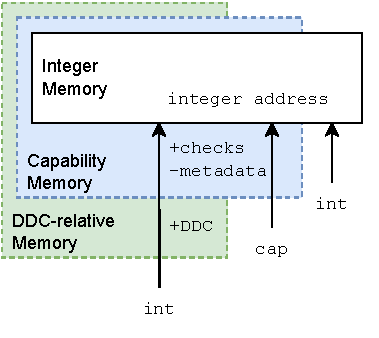
\includegraphics[width=\linewidth]{Figures/cheri_memory.pdf}
      \captionof{figure}{Emulator memory structure}
      \label{fig:emulatormemory}
    \end{minipage}\hfill%
    \begin{minipage}[c]{7.5cm}
        \centering
        {

        \small
      \begin{algorithmic}
        \If{new CHERI instruction}
            \State handle with \code{XCheri64}
        \ElsIf{basic \code{rv64} instruction}
            \If{in capability encoding mode}
                \State handle with \code{Rv64imCapabilityMode}
            \Else{}
                \State wrap memory with DDC-relative
                \State handle with \code{Rv64im}
            \EndIf{}
        \ElsIf{vector instruction}
            \If{in capability encoding mode}
                \State handle with vector unit
            \Else{}
                \State wrap memory in DDC-relative
                \State handle with vector unit
            \EndIf{}
        % \ElsIf{CSR instruction}
        %     \State handle with CSR module
        \EndIf{}
    \end{algorithmic}
        }
    \captionof{figure}{Example algorithm for emulating \code{rv64imvxcheri}}\label{fig:module_algorithm}
    \end{minipage}
\end{figure}

The capability model presented by the C/Rust library has one flaw.\label{safetaggedcap}
Each \code{CcxCap} instance stores capability metadata (e.g. the uncompressed bounds) as well as the compressed encoding.
This makes it potentially error-prone to represent untagged integer data with \code{CcxCap}, as the compressed and uncompressed data may not be kept in sync and cause inconsistencies later down the line.
\code{CcxCap} also provides a simple interface to set the tag bit, without checking whether that is valid.
The emulator introduced the \code{SafeTaggedCap} to resolve this: a sum type which represents either a \code{CcxCap} with the tag bit set, or raw data with the tag bit unset.
This adds type safety, as the Rust compiler forces every usage of \code{SafeTaggedCap} to consider both options, preventing raw data from being interpreted as a capability by accident and enforcing Provenance.

% i.e. doing capability relocation
The final hurdle was the capability relocations outlined in \cref{chap:bg:subsec:cherirelocs}.
Because we're emulating a bare-metal platform, there is no operating system to do this step for us.
A bare-metal C function has been written to perform the relocations\footnote{\gitfile{src/crt_init_globals.c}{CTSRD-CHERI/device-model}{https://github.com/CTSRD-CHERI/device-model/blob/88e5e8e744d57b88b0dbb8e3456ee0e69afc143b/src/crt_init_globals.c}}, which could be compiled into the emulated program.
We decided it would be quicker to implement this in the simulator, but
in the future we should be able to perform the relocations entirely in bare-metal C.


\todomark{I wrote a type-safe wrapper class for capabilities, which either represented a valid capability or raw data, unlike the C library which represents a tagged/untagged capability. I should mention that here}

\subsection{Emulating vectors}
% i.e. using addr, provenance split to write agnostic code?

Vector instructions are executed by a Vector ISA module, which stores all registers and other state.
\code{VLEN} is hardcoded as 128-bits, chosen because it's the largest integer primitive provided by Rust that's large enough to hold a capability.
\code{ELEN} is also 128-bits, which isn't supported by the specification, but is required for capabilities-in-vectors (\cref{chap:capinvec}).
Scaling \code{VLEN} and \code{ELEN} any higher would require the creation and integration of new types that were more than 128-bits long.

To support both CHERI and non-CHERI execution pointers are separated into an address and a \emph{provenance}\footnote{The ``original allocation the pointer is derived from''\cite{memarianExploringSemanticsPointer2019}, or in CHERI terms the bounds within which the pointer is valid.}.
The vector unit retrieves an address + provenance pair from the base register, generates a stream of addresses to access, then rejoins each address with the provenance to access memory.
When using capabilities, provenance is defined in terms of the base register e.g. \enquote{the provenance is provided by capability register X}, or defined by the DDC in integer mode\footnote{See \cref{chap:emu:rvv_int_mode} for the reasoning behind this decision.}.
On non-CHERI platforms the vector unit doesn't check provenance.

Arithmetic and configuration instructions are generally simple to implement, so aren't covered here.
The emulator splits vector memory accesses into three phases: decoding, checking, and execution.
A separate decoding stage may technically not be necessary in hardware (especially the parts checking for errors and reserved instruction encodings, which a hardware platform could simply assume won't happen), but it allows each memory access instruction to be classified into one of the five archetypes outlined in \cref{chap:bg:sec:rvvmemory}.
It is then easy to define the checking and execution phases separately for each archetype, as the hardware would need to do.

\subsubsection{Decoding phase}\label{chap:hardware:subsec:decoding}
Decoding is split into two steps: finding the encoded \paramt{nf} and \paramt{eew} values, then interpreting them based on the encoded archetype.
% Vector memory accesses are encoded under the F extension's Load and Store major opcodes, which already encodes an element width.
Vector memory access instructions are encoded similarly to the F extension's floating-point load/store instructions, which include an ``element width''.
The vector extension adds four extra ``element width'' values which imply the access is vectorized.
% This element width is used to differentiate between vector accesses and scalar floating-point accesses, where a vector access can have one of four widths (8, 16, 32, 64).
If any of these values are found, the instruction is interpreted as a vector access and \paramt{nf} is extracted.
% \paramt{nf} is encoded consistently in all vector memory access instructions

Once the generic parameters are extracted, the \paramt{mop} is checked to determine the indexing method (Unit, Strided, Indexed-Ordered, or Indexed-Unordered).
If a unit access is selected, the second argument field encodes an extra value to choose between different unit-stride archetypes (normal unit access, fault-only-first, whole register, or bytemask).
Strided and indexed accesses just use their dedicated archetypes.
Once the archetype is found, supplemental calculations can be performed (e.g. computing \code{EVL = ceil(vl/8)} for bytemask accesses), and the relevant information is returned as a \code{DecodedMemOp} enumeration.

\todomark{diagram of floating point ld/st vs. vector ld/st}
\todomark{Decision tree for operation decoding}

\subsubsection{Fast-path checking phase}\label{chap:hardware:subsec:checking}
The initial motivation for this project was investigating the impact of capability checks on performance.
We investigate an approach using a \enquote{fast-path}, where certain instructions could check their whole access range against a capability immediately rather than check each individual element.
Other approaches, such as optimizing a parallel checker for $n$ elements, were too hardware-specific and couldn't be modelled in software as well.
\cref{chap:hardware:sec:fastpath} describes methods for calculating the \enquote{tight bounds} for each access type, i.e. the minimum range of bytes that must be accessible, and ways that architectural complexity can be traded off to calculate \emph{wider} bounds.

The emulator calculates tight bounds for all accesses.
If this bounds doesn't pass the capability check, the emulator raises an imprecise trap and stops immediately.
In the case of fault-only-first loads, where synchronous exceptions (e.g. capability checks) are explicitly handled, the access continues regardless and elements are checked individually.
This is also the expected behaviour if a capability check for \emph{wider} bounds fails.
The emulator deviates from the spec in that \code{vstart} is \emph{not} set when the tight bounds check fails, as it does not know exactly which element would have triggered the exception.
As noted in \cref{chap:hardware:sec:fastpath}, a fully compliant machine must check each access to find \code{vstart} in these cases.

\subsubsection{Execution phase}\label{chap:hardware:subsec:execution}
If the fast-path check deems it appropriate, the emulator continues execution of the instruction in two phases.
First, the mapping of vector elements to accessed memory addresses is found.
The code for this step is independent of the access direction, and an effective description of how each type of access works.
It can be found in \todomark{appendix XYZ}.
The previously computed tight bounds are sanity-checked against these accesses, and the accesses are actually performed.

\subsubsection{Integer vs. Capability encoding mode\label{chap:emu:rvv_int_mode}}
As noted in \cref{chap:bg:subsec:cheriencodingmode} CHERI-RISC-V defines two execution modes that the program can switch between.
In Integer mode \enquote{address operands to existing RISC-V load and store opcodes contain integer addresses} which are implicitly dereferenced relative to the default data capability, and in Capability mode those opcodes are modified to use capability operands.
Integer mode was included in the interests of maintaining compatibility with legacy code that hasn't been adapted to capabilities.
As similar vector code may also exist, CHERI-RVV treats vector memory access instructions as \enquote{existing RISC-V load and store opcodes} and requires that they respect integer/capability mode.
\section{Fast-path calculations\label{chap:hardware:sec:fastpath}}
Because CHERI, and indeed the vector extension, target all levels of computer architecture from embedded systems to cloud servers, it's important for fast-paths to be scalable and adjust to the implementation complexity.
To that end, we propose a method of generating the address range for accesses of each archetype, noting where architectural complexity can be traded off for tighter coverage.

\todomark{fast-path could be split up? i.e. for LMUL = 8, could execute a fast-path for each register in the group rather than all 8 at once}

\subsection{Possible fast-path outcomes}
In some cases, a failed address range check may not mean the access fails.
The obvious case is fault-only-first loads, where capability exceptions may be handled without triggering a trap.
Implementations may also choose to calculate wider bounds for the sake of simplicity, or even forego a fast-path check altogether.
Thus, a fast-path check can have three outcomes depending on the circumstances:
\begin{itemize}
    \item Success - All accesses will succeed
    \item Likely-Failure - At least one access \emph{may} raise an exception
    \item Failure - At least one access \emph{must} raise an exception
    \item Unchecked
\end{itemize}

\todomark{if an address range is calculated then: if capability contains it: SUCCESS else if it was wide or FoF: Likely-Failure else: FAILURE}
\todomark{if an address range isn't calculated: Unchecked}
\todomark{Put the above into an algorithm format}

A Success means no per-access capability checks are required.
Likely-Failure and Unchecked results mean each access must be checked, to see if any of them actually raise an exception.
Unfortunately, accesses still need to be checked under Failure, because both precise and imprecise traps need to report the offending element in \code{vstart}\footnote{In very particular cases, e.g. unmasked unit-strided accesses where \code{nf = 1}, the capability bounds could be used to calculate what the offending element must have been. We believe this is too niche of a use case to investigate further, particularly given the complexity of the resulting hardware.}.

Because all archetypes may have Failure or Likely-Failure outcomes, hardware must provide a fallback slow-path for each archetype which checks/performs each access in turn.
In theory, a CHERI-RVV specification could relax the \code{vstart} requirement for imprecise traps, and state that all capability exceptions trigger imprecise traps.
In this case, only archetypes that produce Likely-Failure outcomes need the slow-path.
However, it is likely that for complexity reasons all masked accesses will use wide ranges, thus producing Likely-Failure outcomes and requiring slow-paths for all archetypes anyway.
Because the Likely-Failure and Failure cases require the slow-path anyway, computing the fast-path can only be worthwhile if Success is the common case.

\newcommand{\vstart}{\code{vstart}}
\newcommand{\vstartactive}{\code{vstart}_{\mathit{active}}}
\newcommand{\evl}{\code{evl}}
\newcommand{\evlactive}{\code{evl}_{\mathit{active}}}
\newcommand{\baseaddr}{\mathit{base}}

\subsection{Masked accesses}
For all masked accesses, masked-out/inactive segments should not trigger capability exceptions.
Therefore, a tight bounds must include only the smallest and largest active segments.
These segments can be found by inspecting the mask vector: either checking each bit in turn or using parallel logic to find the lowest/highest set bits.
Care must be taken with these checks to ensure elements outside the range $[\textit{vstart}, \textit{evl})$ are not counted.

\begin{align}
    \vstartactive{} &= \min(i\ \forall\ \vstart{} \le i < \evl{}\ \text{where}\ \mathit{mask}[i] = 1) \\
    \evlactive{}    &= \max(i\ \forall\ \vstart{} \le i < \evl{}\ \text{where}\ \mathit{mask}[i] = 1) + 1
\end{align}

\subsubsection*{Tradeoffs}
If using parallel logic to find the lowest/highest bits, it could be difficult to account for $[\textit{vstart}, \textit{evl})$.
An implementation could choose to only calculate tight bounds when the mask is fully utilized, i.e. $\textit{vstart} = 0, \textit{evl} = \textit{VLEN}$, and assume wider bounds otherwise.

Accounting for masked accesses at all may not be worth the extra complexity.
Only elements masked off on the edges make any difference, and it may be uncommon for long runs of edge elements to be masked off.
Thus, an implementation could choose to ignore masking entirely when computing the ranges.
This does mean that all failures become Likely-Failure when masking is enabled, because all elements outside the capability bounds may be masked off.

\todomark{iterating over elements may still be more energy-efficient than doing individual capability checks?}

\subsection{Unit accesses}
For unit segmented accesses, which includes fault-only first, the tight address range for an access is simple to calculate.
Whole register and bytemask accesses can simplify this by fixing \code{nf = 1} and \code{eew = 8}.

\begin{equation}
    \baseaddr{} + [\vstartactive{} * \code{nf} * \code{eew}, \evlactive{} * \code{nf} * \code{eew})
\end{equation}
\todomark{Note that the equation is a simplification of strided for \code{stride = nf * eew}}

\subsubsection*{Tradeoffs}
\code{nf} is not guaranteed to be a power of two (except for the whole-register case), so calculating the `tight' address range would require a multiplication by an arbitrary four-bit value between 1 and 8.
If this multiplication is too expensive, implementations could choose to classify all $\code{nf} > 1$ cases as Unchecked.
% \todomark{if nf == 1; as normal; if nf != 1 Unchecked}

Unless extra restrictions are placed on \code{vstart}, calculating the start of this range requires another arbitrary multiplication.
To avoid this one could assume \code{vstart = 0} and treat failures as Likely-Failure for other cases.
%for the calculation, perform the capability check and treat failures as Likely-Failure (because the failure could be due to an element before \code{vstart}).
% \todomark{make it clear that in this case vstart = 0 would still be a complete failure}
Once could also classify all nonzero \code{vstart} accesses as Unchecked.
% \todomark{if vstart == 0 failure = failure; if vstart != 0 all = Likely-Failure}

Even if the previous two optimizations are applied, the final range still requires a multiplication $\evl{} * \code{eew}$.
Thankfully, because \code{eew} may only be one of four powers-of-two, this can be encoded as a simple shift.

\subsection{Strided accesses}
Strided accesses bring further complication, especially as the stride may be negative.

\begin{equation}
\mathit{bounds}(\code{stride}) = \baseaddr{} + \left\{
    \begin{array}{ll}
          [\vstartactive{} * \code{stride}, (\evlactive{} - 1) * \code{stride} + \code{nf} * \code{eew}) & \code{stride} \ge 0 \\
          
          [(\evlactive{} - 1) * \code{stride}, \vstartactive{} * \code{stride} + \code{nf} * \code{eew}) & \code{stride} < 0
    \end{array} 
\right.
\end{equation}

This is formed of three components:
\begin{itemize}
    \item $\vstartactive{} * \code{stride}$, the start of the first segment. This can be simplified to 0, just like for unit accesses, to avoid an arbitrary multiplication.
    \item $(\evlactive{} - 1) * \code{stride}$, the start of the final segment. This requires an arbitrary multiplication, unless strided accesses are all Unchecked.
    \item $\code{nf} * \code{eew}$, the length of a segment, which can be implemented with a shift.
\end{itemize}
% Because the stride is not guaranteed to be larger than a segment (or even larger than a single element)

% \todomark{stride may be negative}

\subsection{Indexed accesses}
This is the most complicated access of the bunch, because the addresses cannot be computed without reading the index register.

\begin{align}
    [&\baseaddr{}\ +\ \min(\code{offsets}[\vstartactive{}..\evlactive{}]), \\
    &\baseaddr{}\ +\ \max(\code{offsets}[\vstartactive{}..\evlactive{}])\ +\ \code{nf} * \code{eew})
\end{align}

The most expensive components here are of course $min,\,max$ of the offsets.
These could be calculated in hardware through parallel reductions, making it slightly more efficient than looping over each element.
A low-hanging optimization could be to remove the $\vstartactive{}..\evlactive{}$ range condition, performing the reduction over the whole register group, which would make failures Likely-Failure where $\vstartactive{}\ !=\ 0\ ||\ \evlactive{}\ !=\ \code{VLMAX}$.
This calculation could also be restricted to certain register configurations to reduce the amount of required hardware.
Indeed, the amount of hardware could be reduced to zero by simply classifying all indexed accesses as Unchecked.
\section{Going beyond the emulator}
The emulator is a single example of a conformant CHERI-RVV implementation, and does not exercise every part of the specification.
Four properties stand out:
\begin{itemize}
    \item The emulator assumes all element accesses are naturally aligned, but the spec allows misaligned accesses.
    \item The emulator doesn't consider multiple hardware threads, essentially assuming all accesses are atomic.
    \item Segments/elements are always accessed in order, despite the spec not enforcing ordering
    \item Imprecise traps are used for all exceptions - precise trap behaviour is not explored.
\end{itemize}
This section notes how relaxed access ordering and precise exceptions may affect the hardware in ways not previously explored.

\subsection{Misaligned accesses}
Implementations are allowed to handle vector accesses that are not aligned to the size of the element.
This support is independent of misaligned scalar access support, so if e.g. misaligned 64-bit scalar accesses are allowed, misaligned vector accesses of 64-bit elements do \emph{not} have to be allowed.

Changing the emulator to allow misaligned accesses of integer data would not have any impact on CHERI correctness.
Capability loads/stores must be aligned to \code{CLEN}\cite[Section 3.5.2]{TR-951}, and an implementation cannot change this.
Writing misaligned integer values across a \code{CLEN} boundary would need to make sure to zero the tag bit on both regions, but this applies to scalar implementations as much as vector ones.
Alignment only impacts CHERI-RVV to the extent that it impacts capabilities-in-vectors (\todoref{capinvec - alignment requirements}).

\subsection{Atomicity of accesses/General memory model}
Vector memory instructions are specified to follow the RISC-V Weak Memory Ordering model\todocite{RVV}\footnote{Behaviour under the Total Store Ordering extension hasn't been defined.}, although this model hasn't been fully explained in terms of vectors yet.
RVWMO defines a global order of \enquote{memory operations}: atomic operations that are either loads, stores, or both\todocite[Chapter 14]{RISCV spec}.
The RVWMO spec assumes all memory instructions create exactly one memory operation but calls out that once the vector model is formalized, vector accesses may be defined to create multiple operations.

The RVV spec states \enquote{vector misaligned memory accesses follow the same rules for atomicity as scalar misaligned memory accesses}, i.e. that misaligned accesses may be decomposed into multiple memory operations of any granularity\footnote{e.g. each byte could be written in a separate access.}.
This is the only mention of atomicity in that document.

Again, atomicity of integer data doesn't really impact the fusion of CHERI and RVV, as long as tag bits are correctly zeroed on all integer writes.
However, it does impact capabilities-in-vectors (\todoref{capinvec - atomicity}).

\subsection{Relaxed access ordering and precise traps}
Ordering is only enforced insofar as it is observable.
The only instructions that are forced to perform their accesses in order are indexed-ordered accesses, which can be used to write to e.g. I/O regions where order matters, and instructions that trigger precise traps.
Precise traps require \code{vstart} to be set to a value such that all elements before \code{vstart} have completed their accesses, and all accesses on/after \code{vstart} have not completed or are idempotent.

If a vector memory access instruction is 1. not indexed-ordered and 2. guaranteed not to trigger a precise trap\footnote{Even instructions that \emph{would} trigger precise traps but are guaranteed not to throw an exception or respond to asynchronous interrupt may execute out of order.} then it may execute out of order.
This does not affect CHERI-RVV in any way.
\section{Testing hypotheses}

\hypsubsection{hyp:hw_cap_as_vec_mem_ref}{Feasibility}
This is true.
All vector memory access instructions index the scalar general-purpose register file to read the base address, and CHERI-RVV implementations can simply use this index for the scalar capability register file instead.
This can be considered through the lens of adding CHERI to any RISC-V processor, and in particular adding Capability mode to adjust the behaviour of legacy instructions.
RVV instructions can have their behaviour adjusted in exactly the same way as the scalar memory access instructions.

That approach then scales to other base architectures that have CHERI variants.
For example, Morello's scalar Arm instructions were modified to use CHERI capabilities as memory references\cite[Section 1.3]{armltdMorelloArchitectureReference2021}, so one may simply try to apply those modifications to e.g. Arm SVE instructions.
This only works where Arm SVE accesses memory references in the same way as scalar Arm instructions did i.e. through a scalar register file.

Arm SVE has some addressing modes like \code{u64base}, which uses a vector as a set of 64-bit integer addresses\cite{armltdArmCompilerScalable2019}.
This has more complications, because simply dereferencing integer addresses without a capability is insecure.
Would a CHERI version convert this mode to use capabilities-in-vectors, breaking compatibility with legacy code that expects integer references?
Another option would be to only enable this instruction in Integer mode, and dereference relative to the DDC.
It's possible to port this to CHERI, but requires further investigation and thought.

\hypsubsection{hyp:hw_cap_bounds_checks_amortized}{Fast-path checks}
This is also true, at least for Successful accesses.
Because the RVV spec requires that the faulting element is \emph{always} recorded\cite[Section 17]{specification-RVV-v1.0}, a Failure due to a capability violation requires elements to be checked individually.
CHERI-RVV could change the specification so the faulting element doesn't need to be calculated, which would make Failures faster, but that still requires Likely-Failures to take the slow-path.

There are many ways to combine the checks for a set of vector elements, which can take advantage of the range constraints.
For example, a unit-stride access could a hierarchy of checks: cache-line checks until a Likely-Failure, then tight $m$-element bounds until a Likely-Failure, then the slow-path.
However, the choice of fast-path checks is inherently a trade-off between latency, area, energy usage, and more.
Picking the right one for the job is highly dependent on the existing implementation, and indeed an implementation may decide that parallel per-element checks is better than a fast-path.


\end{document}


%%%%%%%%%%%%%%%%%%%%%%%%%%%%%%%%%%%%%%%%%%%%%%%%%%%%%%%%%%%%%%%%%%%%%%%%%%%%%%%%
%% Main Chapter
%%
\documentclass[../thesis]{subfiles}
\begin{document}

\chapter{The CHERI-RVV software stack\label{chap:software}}
This chapter explores the current state of the CHERI-RVV software stack: mainstream compiler support for vanilla RVV (\cref{chap:software:sec:compilersupport}) and the modifications required to bring support to CHERI-Clang (\cref{chap:software:sec:chericlang}).
The software hypotheses are tested with this knowledge (\cref{chap:software:sec:hypotheses}), and we recommend a set of changes to bring CHERI-Clang support to par with other compilers (\cref{chap:software:sec:chericlangchanges}).
% First, the available compiler support for vanilla RVV is explored and briefly compared to Arm SVE .
% that translates to CHERI-Clang and what changes were necessary to implement capabilities, and 

\section{Compiling vector code}\label{chap:software:sec:compilersupport}
Modern compilers provide many ways to generate vectorized code.
While this support is very advanced for well established vector models, like x86-64 AVX, newer vector models like RVV don't have as many options.
It can even be difficult to get the compiler to generate any vector instructions at all.
This section examines support across the Clang and GCC compilers for various vectorization methods on RVV.

\subsection{Available compilers}
% Before you can compile vector code, the compiler must be told to use a vector ISA.
Compiler support for RVV varies.
On Clang 13 and other LLVM-13-based compilers, version 0.1(?\footnote{It is difficult to verify the actual corresponding version, because there is no readily available specification for v0.1, and the extension supports instructions only present from v0.8 such as whole register accesses.}) of the vector specification is supported as an experimental extension.
Clang/LLVM~14 and up support RVV v1.0.
GCC is an interesting case --- there is a version based on RISC-V GCC 10.1 that partially supports RVV (see \cref{compilerdifferences}), but it was left untouched for a year and deleted as of 17th May 2022.
See \cref{appx:building_rvv_gcc_toolchain} for more information on finding and building this version, and \cref{tab:rvv_cmdline_nocheri} for the required command-line arguments to enable RVV.

\subsection{Automatic vectorization}
\todomark{Figure page showing generated ASM for increment loop - see godbolt links MD}
Compilers with auto-vectorization can automatically create vectorized code from a scalar program.
For example, a scalar loop over an array that increments each element could be converted to a vectorized loop that increments multiple elements at once.
% Although this is simple in some cases, auto-vectorization can take significant effort and time to implement (for example, GCC started implementing it for x86 in 2003 and only turned on basic support in 2007\footnote{\url{https://gcc.gnu.org/projects/tree-ssa/vectorization.html}}).
Clang and GCC support auto-vectorization in Arm SVE, explored further in \cref{chap:soft:compiling:armsve}, but don't yet support it for RVV.
Arm SVE and RVV are quite similar, so there shouldn't be anything blocking auto-vectorization for RVV, it just requires engineering effort.
% There's nothing preventing RVV auto-vectorization, especially as the similar Arm SVE model has auto-vectorization (see \cref{chap:soft:compiling:armsve}), but currently Clang and GCC do not support it.
% Currently there is no support for RVV auto-vectorization in Clang or GCC.
% Both compilers have support for Arm SVE auto-vectorization, explored further in \cref{chap:soft:compiling:armsve}.

\subsection{Vector intrinsics}
\enquote{Intrinsics} are functions defined by the compiler that can invoke low-level functionality and instructions directly for a specific architecture.
When automatic vectorization is not available, intrinsics are the next best thing --- they aren't portable across different ISAs, but present a familiar high-level interface (function calls) that gives fine-grained control over instructions.
% RVV provides an intrinsic for each vector instruction.
The compiler then handles low-level decisions like register allocation under the hood, and sometimes may provide extra functionality for ease of use.

RVV has a comprehensive set of vector intrinsics\cite{specification-RVV-intrinsics}.
%, implemented in the aforementioned special version of GCC and Clang~13+.
With these, the general strip-mining loop is easy to construct:
\todomark{example based on \url{https://github.com/riscv-non-isa/rvv-intrinsic-doc/blob/master/examples/rvv_memcpy.c}}
\begin{enumerate}
    \item Use a \code{vsetvl} intrinsic to get the vector length for this iteration.
    \item Allocate vector registers by declaring variables with vector types (e.g. \code{vuint32m8_t} represents 8 registers worth of 32-bit unsigned integers).
    \item Pass the vector length to the computation/memory intrinsics, which operate on the vector variables.
\end{enumerate}

% \todomark{Hammer home that intrinsics aren't reusable across instruction sets? e.g. AVX intrinsics don't work with RISC-V}

\subsection{Inline assembly}
If a compiler doesn't supply complete intrinsics, or if the programmer desires even more control, inline assembly may be used.
The programmer gives a string of handwritten assembly code to the compiler, which is parsed and directly inserted into the output code.
The compiler still has to parse the instruction, but this method does not depend on any intrinsics being present (or functional).
We used this for CHERI-Clang programs, as it could not use intrinsics without crashing.

Inline assembly can interact with C code and variables through a template syntax.
The programmer inserts a placeholder in the assembly code with a corresponding expression, noting how the expression is stored using a \enquote{constraint}.
For our purposes, constraints enforce that a value is either in a register or in memory.
% As an example, writing to a memory address stored in a variable could use a constraint \code{"m"(*addr)} - i.e. \enquote{the value pointed to by \code{addr} is stored in memory}. \todomark{example} \todomark{the previous sentence kinda sucks at getting the point across. Using a constraint forces the compiler to move the value into a register/memory}

Using the constraint, the compiler determines how the expression's value is stored, and inserts a reference to it in the assembly string.
Because this is done before the assembly string is parsed, and isn't immediately type-checked against the assembly instruction, it can lead to some difficult errors.

Clang and GCC support inline assembly for RVV quite well, and even allows the intrinsic vector types to be referenced by assembly templates (thus making the compiler do register allocation instead of the programmer).
The only caveat is that \emph{memory} constraints are not supported by RVV memory accesses.
None of the vector memory access instructions support address offsets, unlike their scalar counterparts.
Clang always treats the \emph{memory} constraint as an offset access, even when that offset is zero, so it adds an offset to the assembly string (\cref{subfig:inline_asm_vector_memory}), making it invalid.
To get around this, one must use the pointer itself with a \emph{register} constraint (\cref{subfig:inline_asm_vector_ptr_reg}).
On CHERI platforms, because pointers must be stored in capability registers, the \emph{capability register} constraint must be used instead (\cref{subfig:inline_asm_vector_cap_reg}).

\begin{figure}[p]
    \centering
    \begin{subfigure}{0.6\textwidth}
        \inputframedminted[gobble=4,firstline=6,lastline=6]{c}{./code/inline_asm.c}
        \caption{Preamble}
    \end{subfigure}

    \begin{subfigure}{0.49\textwidth}
        \inputframedminted[gobble=4,firstline=7,lastline=10]{c}{./code/inline_asm.c}
        \caption{Load scalar from memory}\label{subfig:inline_asm_memory}
    \end{subfigure}\hfill%
    \begin{subfigure}{0.49\textwidth}
        \inputframedminted[gobble=4,firstline=20,lastline=23]{c}{./code/inline_asm.c}
        \caption{Failed attempt to load vector from memory}\label{subfig:inline_asm_vector_memory}
    \end{subfigure}


    \begin{subfigure}{0.49\textwidth}
        \inputframedminted[gobble=4,firstline=32,lastline=35]{c}{./code/inline_asm.c}
        \caption{Load vector from pointer in register}\label{subfig:inline_asm_vector_ptr_reg}
    \end{subfigure}\hfill%
    \begin{subfigure}{0.49\textwidth}
        \inputframedminted[gobble=4,firstline=43,lastline=46]{c}{./code/inline_asm.c}
        \caption{Load vector from capability in register}\label{subfig:inline_asm_vector_cap_reg}
    \end{subfigure}

    \begin{subfigure}{0.6\textwidth}
        \centering
        \inputframedminted[gobble=4,firstline=57,lastline=67]{c}{./code/inline_asm.c}
        \caption{Portable code for CHERI and non-CHERI.\\\code{pure\_capabilities} is a feature added to CHERI-Clang for this project}\label{subfig:inline_asm_vector_portable}
    \end{subfigure}

    \caption{Inline assembly examples\\\url{https://godbolt.org/z/rW9orr66a}}
    \todomark{Change the code font}
\end{figure}

Broadly speaking, inline assembly supports more RVV instructions than intrinsics do.
It is used extensively in the testbench code for the evaluation (\cref{chap:software:eval}) alongside intrinsics where possible.

% the compiler determines where the value of the expression is/should be stored, and inserts a reference to that location in the assembly string.
% The programmer may also control where the expression is stored by setting a \enquote{constraint}.
% This is an extremely useful feature, particularly if 
% Because this is done before the assembly string is parsed, it can lead to some difficult-to-understand errors.

% \begin{table}[h]
%     \centering
%     \begin{tabular}{c|c}
%        "="  & Output - the old value is overwritten. Can be combined with other constraints. \\
%         "r" & Store in a register \\
%         "vr" & Store in a vector register (RVV only) \\
%         "C" & Store in a capability register (CHERI-Clang only) \\
%         "m" & Store in memory \\
%     \end{tabular}
%     \caption{Inline assembly constraints\cite[Section 6.47.2]{UsingGNUCompiler2022}}
%     \label{tab:inline_asm_constraints}
%     \todomark{Beautify this table}
% \end{table}

\pagebreak
\subsection{RVV vs. Arm SVE}\label{chap:soft:compiling:armsve}
\emph{Summarizes \cite{armltdArmCompilerScalable2019}}

Arm SVE uses a similar model to RVV, where the vector length may scale between 128 and 2048\footnote{RVV slightly differs here, as it allows VLEN smaller than 128.} and the instructions are designed to be totally agnostic across different platforms\cite{stephensARMScalableVector2017}.
Arm have released a C language extension to support SVE development (\cite{armltdARMLanguageExtensions2020}), supported by the Arm Compiler for Embedded\footnote{\url{https://developer.arm.com/Tools\%20and\%20Software/Arm\%20Compiler\%20for\%20Embedded}}, Clang, and GCC.
They support all of the previously examined vectorization types.

Auto-vectorization is supported, and the main focus of the user guide is helping the compiler decide whether to auto-vectorize \cite{armltdArmCompilerScalable2019}.
Intrinsics are also supported, and seem to cover all of the SVE instructions, but take a slightly different approach to RVV.
Arm SVE intrinsics do not directly map to available instructions, but aim to \enquote{provide a regular interface and leave the compiler to pick the best mapping to SVE instructions}, while RVV intrinsics (at least for memory) tend to map 1:1 to existing instructions.
Arm's approach gives more flexibility for future extensions, as the same intrinsics could be compiled to new instructions with newer compilers.

Arm SVE also supports inline assembly, but the experience is notably worse than for RVV.
The two standout issues are a lack of register allocation and the use of condition code flags for branching.
Unlike RVV, the intrinsic types for vector values cannot be referenced in inline assembly\cite{stephensARMScalableVector2017}, so all vector registers must be allocated and tracked by the programmer.
Arm SVE's equivalent of \code{vsetvl}, the \code{while} family\cite{armltdARMLanguageExtensions2020}, do not return the number of updated elements, and instead set the condition flags based on how many elements are updated.
Because there is no way to branch based on the condition flags in C, the programmer must manually insert a label for the top of the loop, and a branch to that label (see \url{https://godbolt.org/z/zoWh9jq3o}), which is more error prone than the RVV method.
Examples of Arm SVE code with auto-vectorization, intrinsics, and inline ASM can be found in \todomark{appendix based on \url{https://godbolt.org/z/zoWh9jq3o}}.


\pagebreak
\section{Compiling vector code with CHERI-Clang}\label{chap:software:sec:chericlang}
Current CHERI compiler work is done on CHERI-Clang, a fork of Clang and other LLVM tools that supports capabilities.
It's based on LLVM~13, so it includes support for vanilla RVV v0.1, but none of the vector-extension related code had been updated to work with capabilities.
This section outlines the changes one has to make to CHERI-Clang and vector code to compile programs for CHERI-RVV.
The required command-line options for CHERI-Clang are shown in \cref{tab:rvv_cmdline_cheri}.

\subsection{Adapting vector assembly instructions to CHERI}\label{addingtochericlang}
LLVM uses a domain-specific language to describe the instructions it can emit for a given target.
The RISC-V target describes multiple register sets that RISC-V instructions can use.
Vanilla RVV vector memory accesses use the General Purpose Registers (GPR) to store the base address of each access.
CHERI-Clang added a GPCR set, i.e. the General Purpose Capability Registers.
As noted in \cref{chap:emu:rvv_int_mode} CHERI-RVV requires the vector memory accesses to support integer \emph{and} capability mode, therefore two versions of the vector accesses must be created: versions which take a capability base address, only available in CHERI/Capability mode, and versions which take integer base addresses for Integer mode.

\todomark{Appendix on how this was done?}
With the above changes, inline assembly could be used to insert capability-enabled vector instructions\todomark{Example}.
However, as this requires using a capability register constraint for the base address, inline assembly code written for CHERI-RVV is not inherently compatible with vanilla RVV.
For un-annotated pointers (e.g. \code{int*}), which are only capabilities in pure-capability code and integers in legacy or hybrid code, a conditional macro can be used to insert the correct constraint: \todomark{example}.
However, this falls apart in hybrid code for manually annotated pointers (e.g. \code{int* \_\_capability}) because the macro cannot detect the annotation.


\subsection{Adapting vector intrinsics to CHERI}
Vector intrinsics are another story entirely.
When compiling for pure-capability libraries, all attempts to use vector intrinsics crash CHERI-Clang \todomark{example of error message?}.
This is due to a similar issue to inline assembly: the intrinsics (both the Clang intrinsic functions and the underlying LLVM IR intrinsics) were designed to take regular pointers and cannot handle it when capabilities are used instead.
\todomark{Appendix which covers what I know so far about this problem?}
Unfortunately the code for generating the intrinsics on both levels is spread across many files, and there's no simple way to change the associated pointer type (much less changing it for pure capability vs. hybrid mode).

It seems that significant compiler development work is required to bring vector intrinsics up to scratch on CHERI-Clang.
We did experiment with creating replacement wrapper functions, where each function tried to mimic an intrinsic using inline asssembly.
These were rejected for two reasons: the increased overhead of a function call on every vector instruction\footnote{This could have been eliminated by using preprocessor macros instead of real functions, but they are difficult to program and do not easily support returning values like intrinsics do.}, and the lack of support for passing vector types as arguments or return values.
The RISC-V ABI treats all vector registers as temporary and explicitly states that \enquote{vector registers are not used for passing arguments or return values}\cite{specification-RISCV-ABI-v1.0rc2}, and CHERI has its own issues with saving vector registers on the stack.

\todomark{segue into saving registers on stack doesn't make sense - doesn't explain why someone would want to}

\subsection{Storing scalable vectors on the stack}
If a program uses more data than can fit in registers, or calls a function which may overwrite important register values, the compiler will save those register values to memory on the stack.
Because vector registers are temporary, and thus may be overwritten by called functions, they must also be saved/restored from the stack\todomark{Example https://godbolt.org/z/KPTW7rcvY}.
This also applies to multiprocessing systems where a process can be paused, have the state saved, and resume later.
RVV provides the whole-register memory access instructions explicitly to make this process easy.

CHERI-Clang contains an LLVM IR pass\footnote{llvm/lib/CodeGen/CheriBoundAllocas.cpp} which enforces strict bounds on so-called ``stack capabilities'' (capabilities pointing to stack-allocated data), which by definition requires knowing the size of the data ahead of time.
This pass assumes all stack-allocated data has a static size, and crashes when dynamically-sized types e.g. scalable vectors are allocated.
It is therefore impossible (for now) to save vectors on the stack in CHERI-Clang, although it's clear that it's theoretically possible.
For example, the length of the required vector allocations could be calculated based on \code{VLEN} before each stack allocation is performed, or if performance is a concern stack bounds for those allocations could potentially be ignored altogether.
These possibilities are investigated further in the next section.

\todomark{Note: Arm Language C extensions https://developer.arm.com/documentation/100987/0000/ defines the concept of a sizeless type, which may be stored on the stack. Would be a good base for RVV?}

\todomark{LLVM IR pass is investigated in TR-949 \$3.8.2, worth noting somewhere}

\pagebreak
\section{Evaluating hypotheses}\label{chap:software:sec:hypotheses}

\hypsubsection{hyp:sw_vec_legacy}{Compiling/running legacy code in integer mode}
This is true for CHERI-RVV, when running the compiled programs in integer mode, as long as the programs only access memory within the DDC.

All vanilla RVV instructions have counterparts with identical encodings and behaviour in CHERI-RVV integer mode, assuming the accessed addresses are all accessible through the DDC.
There are no changes to instruction behaviour that require the compiler's handling of them to change, so a non-CHERI compiler and an integer-mode-CHERI compiler can always produce the same vector instructions from the same code.
This does not apply to capability-mode-CHERI, because integer addressing is not supported in capability-mode-CHERI-RVV.

All legacy vector programs should produce equivalent binaries when compiled for integer-mode-CHERI.
On top of that, all binaries compiled for non-CHERI RVV platforms should produce the same results when run on an equivalent integer-mode-CHERI RVV platform.
Both claims assume the program doesn't perform accesses that \todomark{violate? exceed?} the DDC.

\hypsubsection{hyp:sw_pure_compat}{Converting legacy code to pure-capability code}
This is true for CHERI-RVV, but cannot be done in practice yet.
Some engineering effort is required to support this in CHERI-Clang.
Because this argument concerns source code, all three ways to generate CHERI-RVV instructions must be examined.

\subsubsection*{Inline Assembly --- Unlikely}
For GCC-style inline assembly, it is currently impossible for integer-addressed RVV source code to be recompiled in pure-capability mode without modification.
Integer-addressed RVV assembly uses general-purpose registers for the base address, but the pure-capability instructions require capability registers instead.
The base address register can either be specified directly, so must be changed to a capability register; or specified using template syntax and an ``r'' constraint, which must be changed to a capability ``C'' constraint (\cref{fig:inlineasm,fig:inlineasmcheri}).
Using a preprocessor macro in the template syntax (e.g. \cref{subfig:inline_asm_vector_portable}) could make code portable between non-CHERI and CHERI, but adding it still requires source code changes.

In theory, one could change the behaviour of inline assembly to automatically convert general purpose registers/constraints to capability versions in specific circumstances.
However, this can have wide-reaching ramifications, potentially making code more difficult to understand, or even breaking existing code.

\subsubsection*{Intrinsics --- Yes}
The current specification for RVV intrinsics uses pointer types for all base addresses\cite{specification-RVV-intrinsics}.
In pure-capability compilers all pointers should be treated as capabilities instead of integers, including those in intrinsics.
All RVV memory intrinsics have equivalent RVV instructions, which all use capabilities in pure-capability mode, so changing the intrinsics to match is valid.

Assuming all base address pointers are created in a valid manner (e.g. through \code{malloc} or monotonic decrease, and not through integer literals), the conversion to pure-capability should make them all valid capabilities which are compatible with the intrinsics.
Therefore well-behaved code using RVV intrinsics should be compilable in pure-capability mode without changes.

This is not currently the case for CHERI-Clang, as RVV memory access intrinsics are broken, but this can be fixed with engineering effort.

\subsubsection*{Auto-vectorization --- Yes}
All vanilla RVV instructions have counterparts with identical encodings and behaviour in CHERI-RVV pure-capability mode, assuming the base addresses can be converted to valid capabilities.
Any scalar code that can be 
\begin{enumerate*}[label=\alph*)]
    \item compiled in scalar pure-capability mode\footnote{This ensures all memory accesses use valid capabilities.}, and
    \item auto-vectorized by a legacy RVV compiler,
\end{enumerate*}
must have an equivalent pure-capability vectorized form.
This form could be acquired by performing the auto-vectorization in legacy mode, ensuring all base addresses are available as capabilities, then making the vector instructions use those capabilities.
Therefore a pure-capability compiler can always auto-vectorize CHERI-compliant scalar code if some legacy compiler can also auto-vectorize it.

This is not currently possible for CHERI-Clang, as RVV auto-vectorization is not implemented yet.
Similar models (e.g. Arm SVE) already have auto-vectorization, so RVV auto-vectorization (and thus CHERI-RVV auto-vectorization) should be possible.

\hypsubsection{hyp:sw_stack_vectors}{Saving vectors on the stack}
% \todomark{Yes vectors can be stored on the stack}
This is true in theory, but not yet supported by CHERI-Clang in practice.
Placing variable-length structures on the stack is possible as long as the length can be known at runtime (and as long as the stack has space, of course).
This isn't exclusive to CHERI --- to push and pop values on the stack, the stack pointer must be incremented or decremented by the size of the value.
Because the length already has to be measured, and CHERI-RISC-V supports setting capability bounds from runtime-computed values, it's entirely possible to correctly set tight bounds for capabilities pointing to variable-length vectors on the stack.

% Arm SVE explicitly defines a ``sizeless type'' in the C language extensions \cite{} that may be stored on the stack, so this will need to be implemented for 
% \todomark{Note: Arm Language C extensions https://developer.arm.com/documentation/100987/0000/ defines the concept of a sizeless type, which may be stored on the stack. Would be a good base for RVV?}

A minor complication is presented by a note in TR-949\cite[Section 3.8.2]{TR-949} concerning ``re-materializing bounded stack variables''.
This section implies LLVM can try to re-create a pointer-to-stack at any time with minimal cost, but this may not be able to apply to vectors.
Measuring the bounds requires measuring \code{VLMAX} by changing \code{vl}, which could then require saving/restoring the old value.
This is only a performance issue, and in the worst case we can just say pointers-to-stack-vectors are not re-materializable, so it isn't a dealbreaker.
Further investigation of this issue is left as future work.
% LLVM allows pointers to be non-re-materializable, so this isn't a dealbreaker, but it should be investigated in the future.
% Further investigation of this issue is left as future work.

\hypsubsection{hyp:sw_multiproc}{Running CHERI-RVV code in a multiprocessing system}
% \todomark{H-D: Yes IFF vectors can be stored on the stack. May require a dynamic stack bounds calculation based on VLEN.}
This requires two conditions: an OS must be able to save and restore vector state, and the vector hardware must support resuming from an interrupted state.
The first condition is easy to fulfil by extending the previous hypothesis. 
If it is possible to save variable-length vectors on the stack, given their length is known at runtime, it must also be possible to save their data on the heap.
Some OSs might need to make changes to their ``current process state'' structure to support variable-length data, and they would also need to allocate space for the \code{vtype} value, but it is certainly possible.

The second condition can be upheld in two ways.
First, if the OS only context switches and services interrupts while the vector hardware is in a complete state (i.e. not partially executing an instruction), then context switches and interrupts are completely transparent to the vector hardware and no changes need to be made.
Secondly, if context switches and interrupts can actually interrupt vector instructions partway through, then they can only be cleanly resumed if the vector hardware supports precise traps for the exact instruction being executed.

\subsection{Verification and testing: \code{vector\_memcpy}}\label{chap:software:eval}
To verify the behaviour of the CHERI-RVV instructions, we developed a self-checking test program for the emulator to execute.
At first it was hand-written, but in order to test a wide range of \code{vtype}s we now generate it with a Python script.
It consists of fifty-seven tests of different vector memory access archetypes under various configurations (\cref{tab:vectormemcpyschemes}).

% The test code is compatible with integer-mode and capability-mode CHERI (and non-CHERI) through preprocessor macros, as shown in .
\todomark{Put the compatibility preprocessor stuff in the compiler appendix}
The test code will use intrinsics wherever the compiler supports them (see \cref{compilerdifferences}), and falls back to inline assembly otherwise.
Inline assembly uses the preprocessor macro from \cref{subfig:inline_asm_vector_portable} to handle CHERI and non-CHERI platforms.
% On CHERI platforms, which don't support intrinsics, the preprocessor macro from \todoref{preprocessor macro} is used to support inline ASM.
% Where the compiler supports intrinsics, the test code will use them, and otherwiuse
% Based on the compiler version, the test code runs operations with intrinsics where
% To make up for inconsistent RVV support, the test code checks the compiler version and implements operations with inline assembly or intrinsics as supported.
% Because the compilers don't have consistent RVV support (see \cref{compilerdifferences})

These tests are run under \emph{harnesses}, which provide setup and self-checking code for common cases:
The Vanilla harness tests a simple \code{memcpy} between two arrays;
Masked tests that every other element is copied, not all of them;
Segmented tests a \code{memcpy} into four separate output arrays, each a different field of a four-field structure.
There is also a special test for fault-only-first: FoF loads are performed at the edge of mapped memory, and the test verifies that out-of-bounds exceptions are swallowed and \code{vl} is reduced accordingly.
All tests were successful when they ran, but some testbenches could not be built with some compilers.
The full set of test results is available in \cref{chap:fullresults}.

\begin{table}[h]
    \centering
    \begin{tabular}{lcc}
    \toprule
        Test Scheme & Harness & Compilers \\
    \midrule
        Unit Stride & Vanilla & All \\
        Strided & Vanilla & All \\
        Indexed & Vanilla & All \\
        Whole Register & Vanilla & All \\
        Fault-only-First & Vanilla & All \\
        
        Unit Stride (Masked) & Masked & All \\
        Bytemask Load & Masked & \code{llvm-15} only \\
        
        Unit Stride (Segmented) & Segmented & All \\

        Fault-only-First Boundary & --- & All \\
    \bottomrule
    \end{tabular}
    \caption{\code{vector\_memcpy} test schemes and harnesses}
    \label{tab:vectormemcpyschemes}
\end{table}

\section{Recommended changes for CHERI-Clang}
\begin{itemize}
    \item Build on current work to make all RVV memory access instructions and pseudoinstructions CHERI-compatible.
    \item Make RVV memory access intrinsics take capabilities as arguments when compiled in pure-capability mode.
    \item Consider options on handling stack bounds for scalable vectors, and implement in the CheriBoundAllocas IR pass.
\end{itemize}
% \todomark{where to put something on how CHERI-Clang should change?}


\end{document}


%%%%%%%%%%%%%%%%%%%%%%%%%%%%%%%%%%%%%%%%%%%%%%%%%%%%%%%%%%%%%%%%%%%%%%%%%%%%%%%%
%% Other Chapter
%%
\chapter{Capabilities-in-vectors}

\section{Emulator changes}

\section{Hardware implications}

\section{Possible software improvements}

\section{Testing hypotheses}

\hypsubsection{hyp:cap_in_vec_storage}{Holding capabilities in vectors}
It is possible for a single vector register to hold a capability (and differentiate a capability from integer data) as long as \code{VLEN = CLEN}.
\code{VLEN} could also be larger, and a compliant implementation must then have \code{VLEN} be an integer multiple of \code{CLEN}.
In theory, one could also describe a scheme where capabilities must be held by multiple registers together (e.g. \code{VLEN = CLEN/2} with one tag bit for every two registers), but this would complicate matters.

If an implementation decides, as we did, that elements of width \code{CLEN} are required to produce capabilities, then $\code{VLEN} \ge \code{ELEN}$ therefore $\code{VLEN} \ge \code{CLEN}$.
If a short \code{VLEN} is absolutely essential, one could place precise guarantees on a specific set of instructions to enable it (e.g. \code{SEW=64, LMUL=2} unit-stride unmasked loads could guarantee atomic capability transfers) but the emulator does not consider this.
The CHERI security properties also impose some conditions.

\subsubsection*{Provenance \& Monotonicity}
The tag bit must be protected such that capabilities cannot be forged from integer data.
The emulator's integer/capability context approach, where the tag bit may only be set on copying a valid capability from memory, and the output tag bit is zeroed on all other accesses, enforces this correctly.

\subsubsection*{Integrity}
Integrity is not affected by how a capability is stored, as long as the other properties are maintained.

%%%%%%%%%%%%%%%%%%%%%%%%%%%%%%%%%%%%%%%%%%%%%%%%%%%%%%%%%%%%%%%%%%%%%%%%%%%%%%%%%%%%%%%
\hypsubsection{hyp:cap_in_vec_load_store}{Sending capabilities between vectors and memory}\label{chap:capinvec:hyp_load_store}
For this to be the case, the instructions which can load/store capabilities must fulfil certain alignment and atomicity requirements.
They must require all accesses be \code{CLEN}-aligned, or at least only load valid caps from aligned addresses, because tag bits only apply to \code{CLEN}-aligned regions.
TR-951 states that capability memory accesses must be atomic\cite[Section 11.3]{TR-951}.
This applies to vectors, even in ways that don't apply to scalar accesses.

Individual element accesses for a vector access must be atomic relative to each other.
This is relevant for e.g. a strided store uses a zero or unaligned stride, such that one element writes a valid capability and another element overwrites part of that address range.
In that case, either the second element should ``win'' and clear the tag bit, or the first element should ``win'' and write the full capability atomically.
For the emulator this condition is easily met.

\subsubsection*{Provenance}
Provenance requires the accesses be atomic as described above, and require that tag bits are copied correctly: the output tag bit must only be set if the input had a valid tag bit.
These conditions also apply to scalar accesses.

\subsubsection*{Monotonicity}
These loads/stores do not attempt to manipulate capabilities, so have no relevance to monotonicity.

\subsubsection*{Integrity}
The same conditions for scalar and other vector accesses apply to maintain Integrity: namely that the base capability for each access should be checked to ensure it is valid.
The emulator doesn't allow capabilities-in-vectors to be dereferenced directly, but if an implementation allows it those capabilities would also need to be checked.

%%%%%%%%%%%%%%%%%%%%%%%%%%%%%%%%%%%%%%%%%%%%%%%%%%%%%%%%%
\hypsubsection{hyp:cap_in_vec_manip}{Manipulating capabilities in vectors}
The emulator limits all manipulation to clearing the tag bit, achieved by writing data to the register in an integer context.
In theory, it's possible to do more complex transformations, which can be proven by implementing each vector manipulation on vector elements as sequential scalar manipulations on scalar elements.
With this method, all pre-existing scalar capability manipulations can become vector manipulations, but the utility seems limited.
For example, instructions for creating capabilities or manipulating bounds en masse don't have an obvious use case.
If more transformations are added they should be considered carefully, rather than creating vector equivalents for all scalar manipulations.

\subsubsection*{Provenance \& Monotonicity}
Because the only possible manipulations clear the tag bit, it's impossible to create or change capabilities, so Provenance and Monotonicity cannot be violated.
Any manipulations that create capabilities, or potentially any manipulations that transfer capabilities from vector registers directly to scalar registers, would require more scrutiny.

\subsubsection*{Integrity}
As stated before, capabilities-in-vectors cannot be dereferenced directly, so there is no impact on Integrity.



%%%%%%%%%%%%%%%%%%%%%%%%%%%%%%%%%%%%%%%%%%%%%%%%%%%%%%%%%%%%%%%%%%%%%%%%%%%%%%%%
%% Conclusion (with future work)
%%
\chapter{Evaluation}

\section{Vectorized memcpy test and results}

\section{Capabilities-in-vector test and results}

\section{Conclusion}
\todomark{Summarize hypotheses outcomes}
\todomark{Summarize results}
\todomark{List artifacts - github repositories, where to get the rust-cheri-compressed-cap crate etc}
\label{wc:end}